\documentclass[UTF8,a4paper,11pt,fontset=windows]{ctexart}
\usepackage[left=2cm,right=2cm,top=2.3cm,bottom=2.2cm]{geometry}
\usepackage{amsmath,amssymb,bm}
\usepackage{booktabs,longtable,tabularx,array}
\usepackage{graphicx,float,caption}
\usepackage{xcolor,fancyhdr,enumitem}
\usepackage[hidelinks]{hyperref}
\usepackage{microtype}

\graphicspath{{../figures/}}
\definecolor{navy}{HTML}{17365D}
\definecolor{blue}{HTML}{2F5597}
\definecolor{lightblue}{HTML}{EEF4FB}
\definecolor{textgray}{HTML}{444444}

\ctexset{
  section={format=\Large\bfseries\color{navy},beforeskip=1.2em,afterskip=0.7em},
  subsection={format=\large\bfseries\color{blue},beforeskip=0.9em,afterskip=0.5em}
}
\setlength{\parindent}{2em}
\setlength{\parskip}{0.25em}
\renewcommand{\arraystretch}{1.22}
\setlist[itemize]{leftmargin=2em,itemsep=0.2em,topsep=0.3em}

\pagestyle{fancy}
\fancyhf{}
\fancyhead[L]{\small\color{textgray}量子物理计算方法选讲 · 第三讲作业}
\fancyhead[R]{\small\color{textgray}Hubbard 环上的 Lanczos 方法与谱函数}
\fancyfoot[C]{\small\thepage}
\renewcommand{\headrulewidth}{0.4pt}
\captionsetup{font=small,labelfont=bf,labelsep=quad}
\newcommand{\code}[1]{\texttt{#1}}
\newcommand{\good}{\textcolor{blue}{通过}}

\title{\vspace{2.2cm}\textbf{\Huge\color{navy}第三讲作业}\\[0.6em]
\textbf{\LARGE Hubbard 环上的 Lanczos 方法与谱函数}\\[1.4em]
\large 固定粒子数精确对角化 · Lanczos 三对角化 · 连分数 Green 函数}
\author{量子物理计算方法选讲}
\date{2026-09-29}

\begin{document}
\maketitle
\thispagestyle{empty}
\vfill
\begin{center}
\renewcommand{\arraystretch}{1.35}
\begin{tabular}{>{\bfseries}p{3.2cm}p{10.5cm}}
\toprule
主参数 & $N=8,\ t=1,\ U=4,\ \eta=0.11$，半满 \\
Hilbert 空间 & $U(1)\times U(1)$ 分块，主块 $(N_\uparrow,N_\downarrow)=(4,4)$ \\
谱算法 & 逐格点、逐自旋 Lanczos + 反向连分数 \\
复现入口 & \code{python run\_homework3.py} \\
随机种子 & 20260928 \\
\bottomrule
\end{tabular}
\end{center}
\vspace{1.2cm}
\noindent\colorbox{lightblue}{\parbox{0.94\textwidth}{
\textbf{摘要：}本作业在固定上、下自旋粒子数的块中实现一维周期 Hubbard 模型。
Hamiltonian 的主计算采用 matrix-free 作用，并以独立装配的稀疏矩阵校验。
谱函数由加、减粒子扇区中的 Lanczos 系数和反向连分数得到，不使用全 Hilbert
空间稠密对角化或逐本征态求和。}}
\vfill
\clearpage

\tableofcontents
\clearpage

\section{模型、表示与数值路线}

一维 Hubbard 环的 Hamiltonian 为
\begin{equation}
H=-t\sum_{j,\sigma}\left(c^\dagger_{j\sigma}c_{j+1,\sigma}+\mathrm{h.c.}\right)
  +U\sum_j n_{j\uparrow}n_{j\downarrow},
\end{equation}
格点指标按模 $N$ 取。Hamiltonian 中不加入化学势项；化学势由
\begin{equation}
\mu=\frac12\left[E_0(N+1)-E_0(N-1)\right]
\end{equation}
确定，谱图横轴使用 $\omega-\mu$。

每个自旋种类用一个 $N$ 位整数表示，比特 $j$ 对应格点 $j$。全局轨道顺序固定为
$(0\uparrow,\ldots,N-1\uparrow,0\downarrow,\ldots,N-1\downarrow)$。
施加费米算符时，根据目标轨道之前的已占据数确定符号；跳跃统一写成先湮灭、
再产生，因此周期边界键与普通键使用同一套规则。

固定 $(N_\uparrow,N_\downarrow)$ 后，分别枚举两个定粒子数 bit mask，并建立长度
$2^N$ 的 mask 到块内序号数组，使矩阵元循环中的查找为 $O(1)$。

\subsection{源码结构}
\begin{center}
\begin{tabularx}{0.94\textwidth}{@{}>{\ttfamily\small}p{3.7cm}X@{}}
\toprule
\textbf{文件} & \textbf{职责} \\
\midrule
hubbard\_basis.py & 分块基底、O(1) 查找、费米算符及符号 \\
hubbard\_operator.py & matrix-free Hamiltonian、独立 CSR 矩阵、低能本征对 \\
lanczos.py & Lanczos 递推、三对角矩阵、Ritz 值、反向连分数 \\
spectral.py & 加减粒子向量、目标块、化学势和总态密度 \\
run\_homework3.py & 一次生成全部数据、校检与图 \\
tests/ & 解析基准、交叉表示与故障注入测试 \\
\bottomrule
\end{tabularx}
\end{center}

\section{分块、Hamiltonian 与基态}

主块 $(4,4)$ 的组合公式
\begin{equation}
\dim\mathcal H_{N_\uparrow,N_\downarrow}
=\binom{N}{N_\uparrow}\binom{N}{N_\downarrow}
\end{equation}
与实际枚举维数均为 $4900$。在 $U=4$ 时得到
\begin{equation}
\boxed{E_0=-4.60352629998921},\qquad g_0=1.
\end{equation}

\begin{table}[H]
\centering
\caption{Hamiltonian 与基态的独立校检}
\begin{tabular}{p{8.2cm}rr}
\toprule
校检量 & 实测值 & 结论 \\
\midrule
matrix-free / 独立 CSR 相对作用误差 & $1.2493\times10^{-16}$ & \good \\
$\lVert H-H^\dagger\rVert$ & $0$ & \good \\
$\mathrm{Tr}(H_U)$：期望 / 实测 & $39200/39200$ & \good \\
基态相对残差 & $1.5443\times10^{-14}$ & \good \\
两种表示的 $E_0$ 差 & $2.1316\times10^{-14}$ & \good \\
\bottomrule
\end{tabular}
\end{table}

厄米性只针对单向跳跃或不对称符号；相互作用 trace 的组合恒等式专门检查
$U$ 项。matrix-free 与独立 CSR 的随机复向量比较则覆盖跳跃符号、周期边界、
目标索引和相互作用作用。

\section{Lanczos 三对角化}

从固定随机种子的随机向量出发，递推关系为
\begin{equation}
Hq_m=b_mq_{m-1}+a_mq_m+b_{m+1}q_{m+1}.
\end{equation}
约定 $b_0=0$。前六组系数为：

\begin{table}[H]
\centering
\caption{前六组 Lanczos 系数}
\begin{tabular}{rrrr}
\toprule
$m$ & $a_m$ & $b_m$ & $b_{m+1}$ \\
\midrule
0 & 7.9696938017 & 0 & 4.2473265360 \\
1 & 8.0882816689 & 4.2473265360 & 5.4562485018 \\
2 & 8.1100438218 & 5.4562485018 & 5.8829236759 \\
3 & 8.2947849533 & 5.8829236759 & 6.4975269813 \\
4 & 7.9676999431 & 6.4975269813 & 6.6118019978 \\
5 & 8.0112260463 & 6.6118019978 & 6.6138816472 \\
\bottomrule
\end{tabular}
\end{table}

\begin{equation}
T_6=\begin{pmatrix}
7.9697&4.2473&0&0&0&0\\
4.2473&8.0883&5.4562&0&0&0\\
0&5.4562&8.1100&5.8829&0&0\\
0&0&5.8829&8.2948&6.4975&0\\
0&0&0&6.4975&7.9677&6.6118\\
0&0&0&0&6.6118&8.0112
\end{pmatrix}.
\end{equation}

正交性残差为 $6.850\times10^{-16}$；已完整构造列的 $HQ-QT$ 残差为
$7.891\times10^{-15}$；加入末端 $b_6q_6$ 后，完整递推残差为
$8.262\times10^{-15}$。若起始向量严格等于基态，则第一次去掉
$a_0\lvert\Phi_0\rangle$ 后残差为零，Krylov 空间维数为 1。

\section{连分数与直接求解}

对同一起始向量 $e_0$，计算
\begin{equation}
G(z)=\langle e_0\vert(z-H)^{-1}\vert e_0\rangle
=\cfrac{1}{z-a_0-\cfrac{b_1^2}{z-a_1-\cfrac{b_2^2}{\ddots}}}.
\end{equation}
连分数必须从最深层反向递推并包含最深的 $a_m$。480 步结果为：

\begin{table}[H]
\centering
\caption{连分数与直接稀疏线性求解}
\small
\begin{tabular}{p{2.5cm}p{4.2cm}p{4.2cm}r}
\toprule
$z$ & 连分数 & 直接求解 & 绝对偏差 \\
\midrule
$0.7+0.11i$ & $-0.067064955-0.00052123791i$ & $-0.067064955-0.00052123791i$ & $1.084\times10^{-19}$ \\
$-1.3+0.11i$ & $-0.058888929-0.00039279886i$ & $-0.058888929-0.00039279886i$ & $1.388\times10^{-17}$ \\
$5+0.11i$ & $-0.096795070-0.0034958612i$ & $-0.096795069-0.0034958617i$ & $1.133\times10^{-9}$ \\
\bottomrule
\end{tabular}
\end{table}

$z=5+0.11i$ 更靠近高能谱结构，因此收敛最慢；其误差从 256 步的
$4.834\times10^{-6}$ 降至 480 步的 $1.133\times10^{-9}$。完整步数表收入
\code{output/result.md}。

\section{总态密度、权重与解析基准}

加电子进入 $(5,4)$、$(4,5)$ 块，减电子进入 $(3,4)$、$(4,3)$ 块。
每个格点与自旋均显式求和，并把初始向量的范数 $\alpha^2$ 乘回连分数。
加谱使用 $z=\omega+i\eta+E_0$，减谱使用 $z=-\omega+i\eta+E_0$。

在 $U=4$ 时
\begin{equation}
\boxed{\mu=2,\qquad w_{\mathrm{add}}=8,\qquad w_{\mathrm{rem}}=8}.
\end{equation}
加谱和减谱分别满足半满求和规则。

粒子-空穴对称性直接按
$\rho_{\rm add}(\xi)=\rho_{\rm rem}(-\xi)$ 在对称频率网格上逐点比较，
并以两条谱中较大的峰值归一。$U=0,2,4,6,8$ 的相对最大偏差分别为
$4.521\times10^{-14}$、$5.793\times10^{-8}$、$3.382\times10^{-7}$、
$3.180\times10^{-7}$ 和 $1.577\times10^{-12}$。

\begin{figure}[H]
\centering
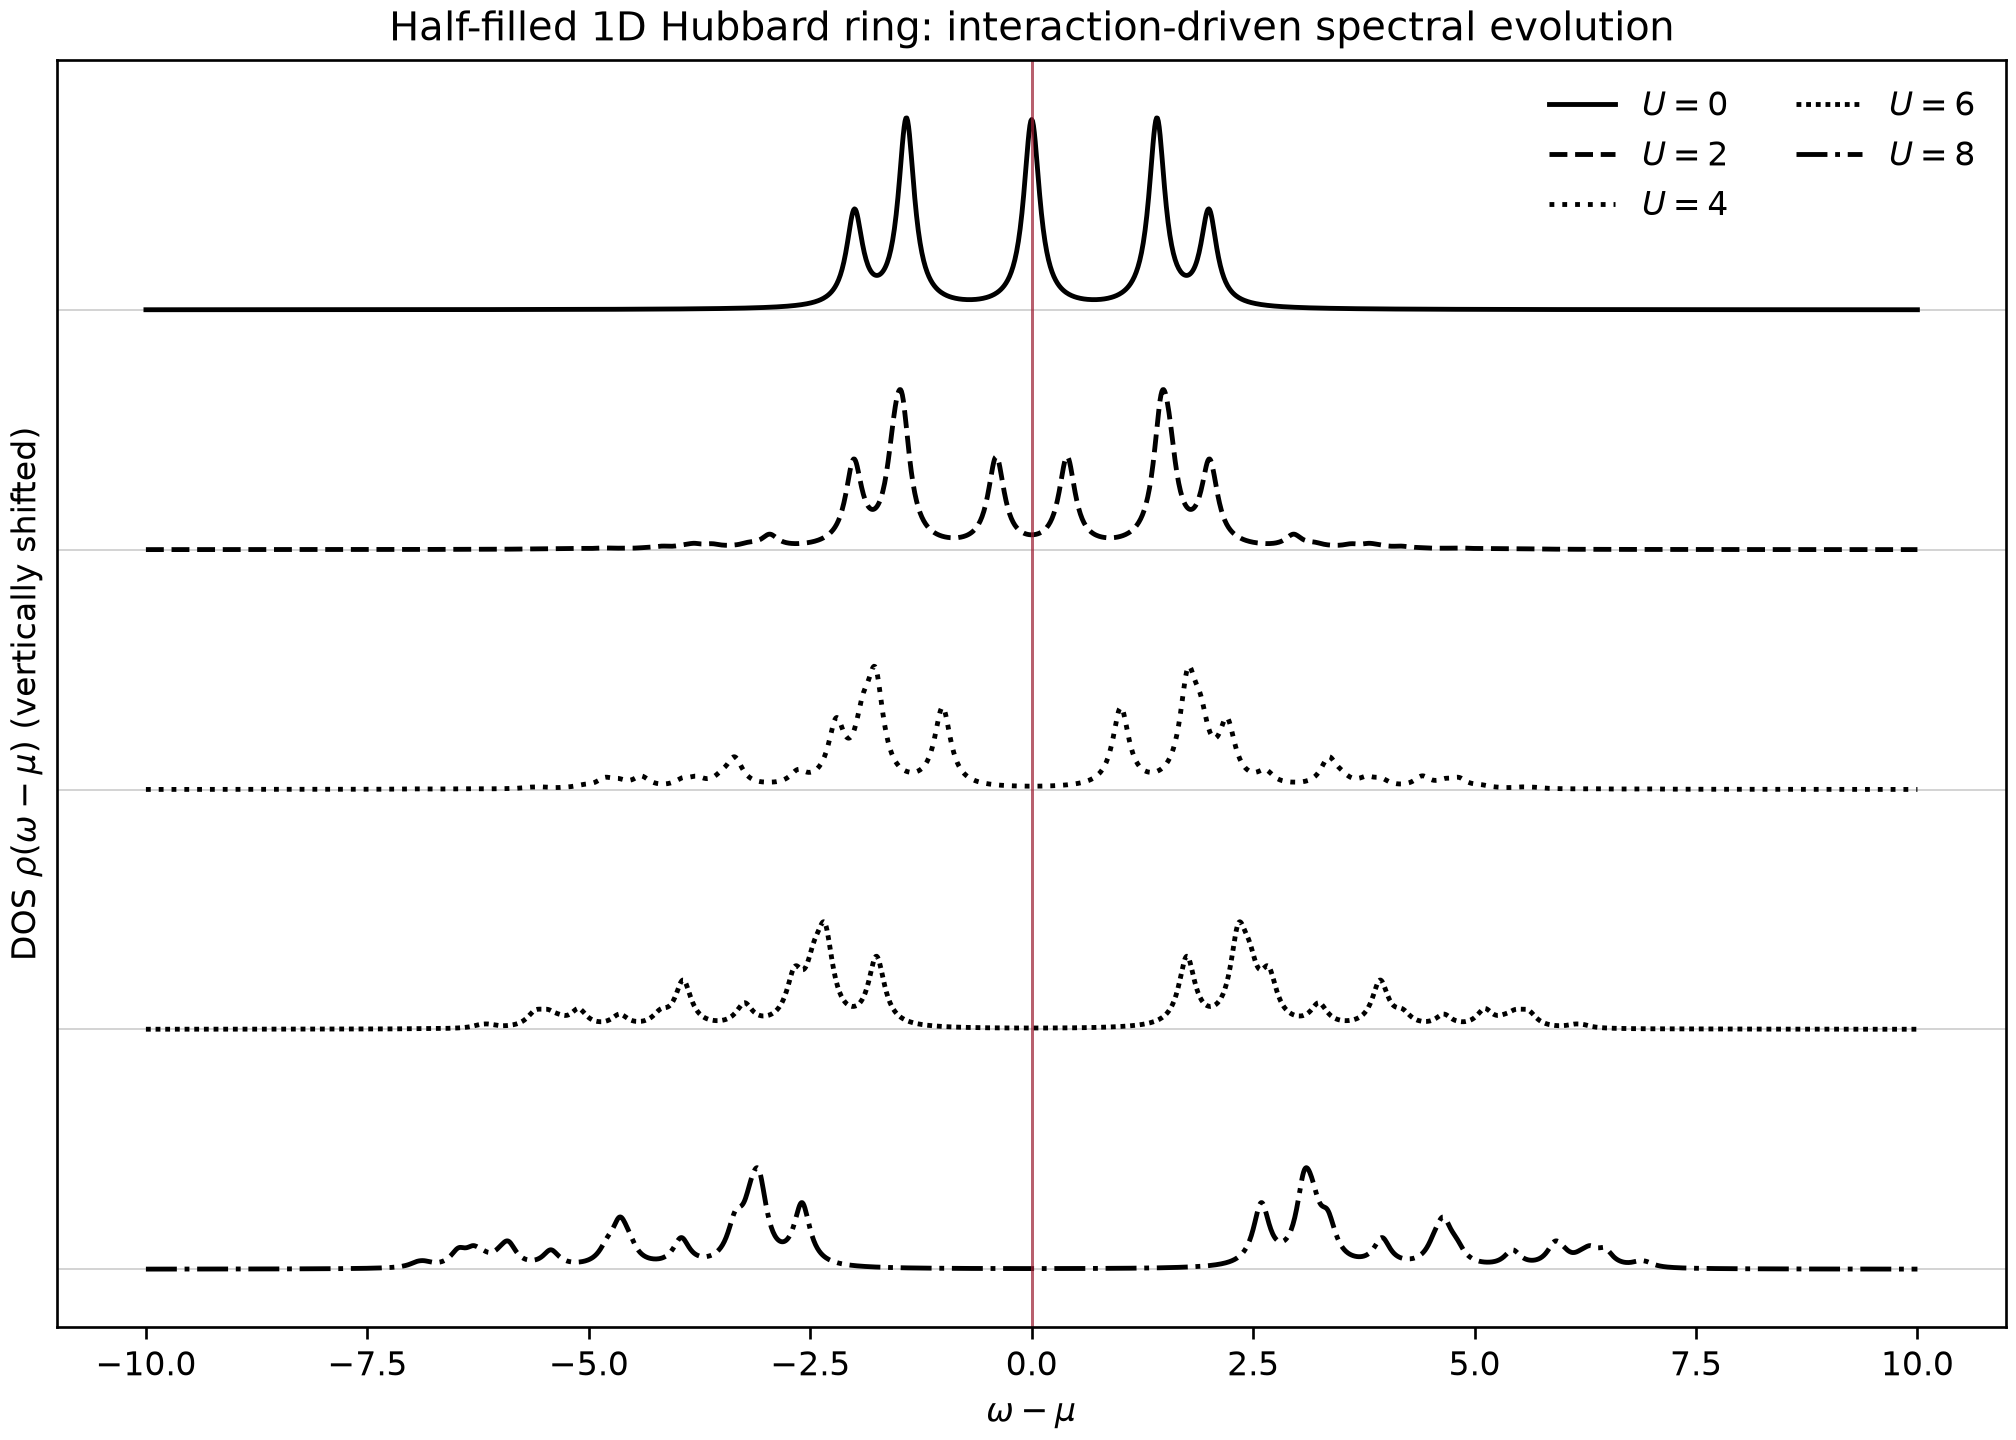
\includegraphics[width=0.98\textwidth]{dos_vs_U_stacked.png}
\caption{$U=0,2,4,6,8$ 的总态密度。各曲线使用同一纵向尺度，仅为可读性作竖直平移；红线为 $\omega-\mu=0$。}
\end{figure}

自由极限的解析谱为
\begin{equation}
\rho(\omega)=2\sum_k\frac{1}{\pi}
\frac{\eta}{(\omega-\epsilon_k)^2+\eta^2},\qquad
\epsilon_k=-2t\cos\frac{2\pi k}{N}.
\end{equation}
数值谱相对于解析峰值归一的最大偏差为
\begin{equation}
\boxed{8.6674\times10^{-14}}.
\end{equation}
该基准同时锁定跳跃能标、周期边界、展宽、总权重、$\alpha^2$ 因子和
连分数递推方向。

\begin{figure}[H]
\centering
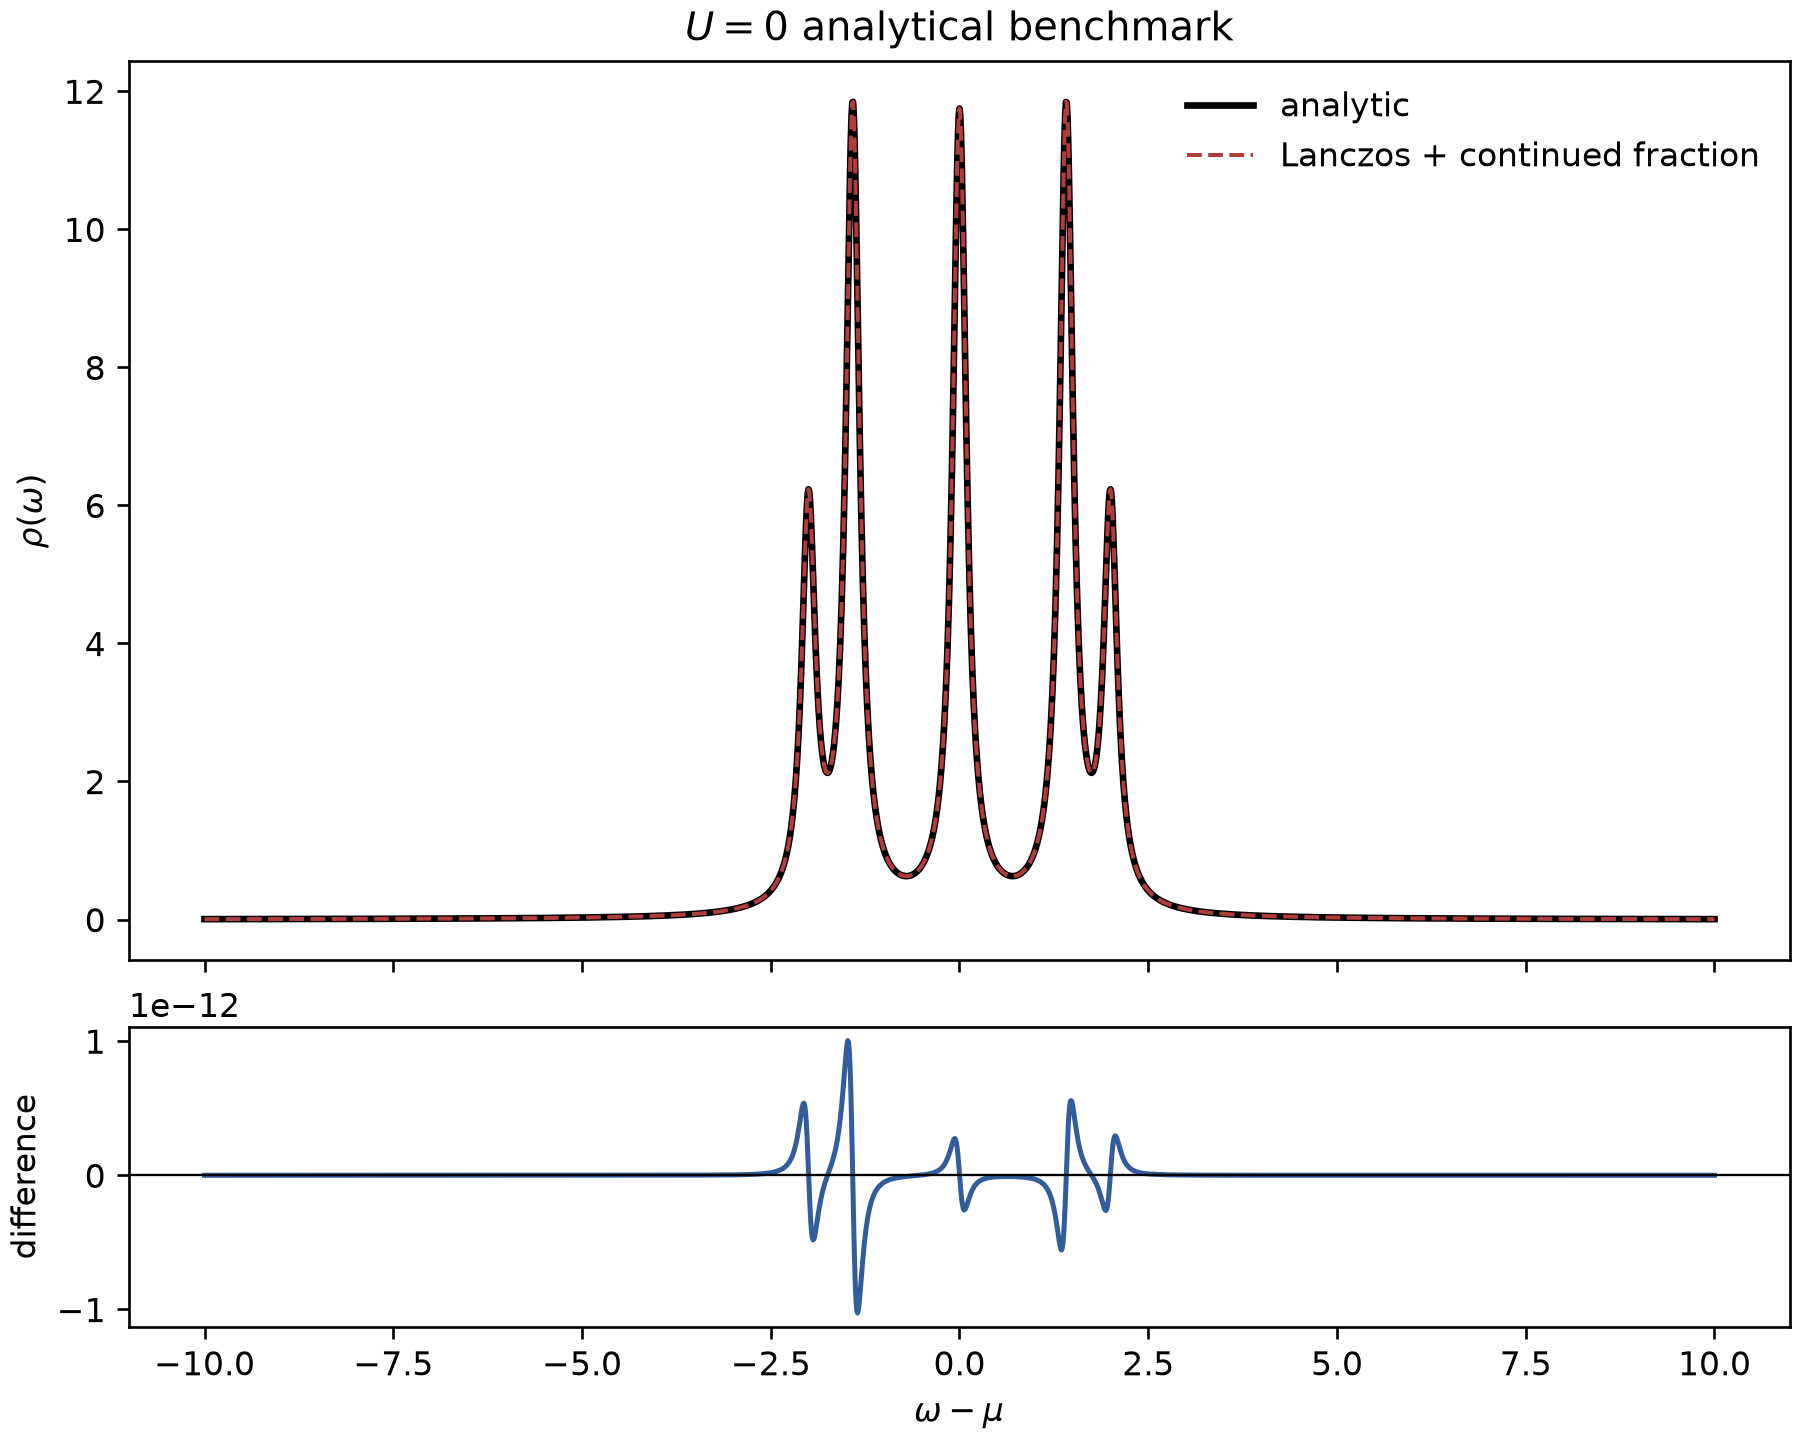
\includegraphics[width=0.96\textwidth]{u0_analytic_benchmark.png}
\caption{$U=0$ 数值谱与自由费米子解析谱的逐点比较。}
\end{figure}

\section{选做结果}

\subsection{简并陷阱}
\begin{table}[H]
\centering
\caption{“一格点 $\times N$”快捷法的原始值与偏离量级}
\begin{tabular}{rrrrrr}
\toprule
$N$ & $U$ & 简并度 & 完整求和 & 快捷法原始值 & 最大偏离 \\
\midrule
8 & 0 & 4 & $8/8$ & $6/10$ & $2.00\times10^{0}$ \\
8 & 4 & 1 & $8/8$ & $8/8$ & 0（机器精度内） \\
\bottomrule
\end{tabular}
\end{table}

完整求和在两个 $N=8$ 算例中均为 $8/8$。原始值 $6/10$ 对应程序在简并基态
空间中选出的当前基矢；换取另一组简并子空间基矢时，这两个分量可能改变，
因此不能把 $6/10$ 当成基矢无关的物理量。表中同时保留相对 $8/8$ 的最大
偏离量级 $2.00\times10^0$，作为不区分偏离落在加谱或减谱一侧的稳健诊断；
该指标仍针对当前选态，并不宣称完全消除简并基矢依赖。作为闭壳层对照，
$N=6,U=0$ 的最大偏离仅为 $8.882\times10^{-16}$。判断准则是检查费米面
是否具有严格正的闭壳层隙，或更一般地检查所选态是否保持平移对称。

\subsection{Mott 谱演化}
\begin{table}[H]
\centering
\caption{化学势处的归一化谱权重}
\begin{tabular}{rrrrr}
\toprule
$U$ & $\rho(0)$ & $\rho_{\max}$ & $\rho(0)/\rho_{\max}$ & $\mu$ \\
\midrule
0 & 11.74902755 & 11.84593085 & 0.991819697 & 0 \\
2 & 0.919488892 & 9.884346144 & 0.093024756 & 1 \\
4 & 0.209671658 & 7.613997057 & 0.027537659 & 2 \\
6 & 0.086398597 & 6.648692822 & 0.012994825 & 3 \\
8 & 0.044751281 & 6.274029512 & 0.007132781 & 4 \\
\bottomrule
\end{tabular}
\end{table}

随 $U$ 增大，化学势附近的谱权重迅速受抑制，权重向低能和高能两侧重新分配。
有限尺寸和 $\eta=0.11$ 的 Lorentzian 展宽使隙内保留非零尾部。

\begin{figure}[H]
\centering
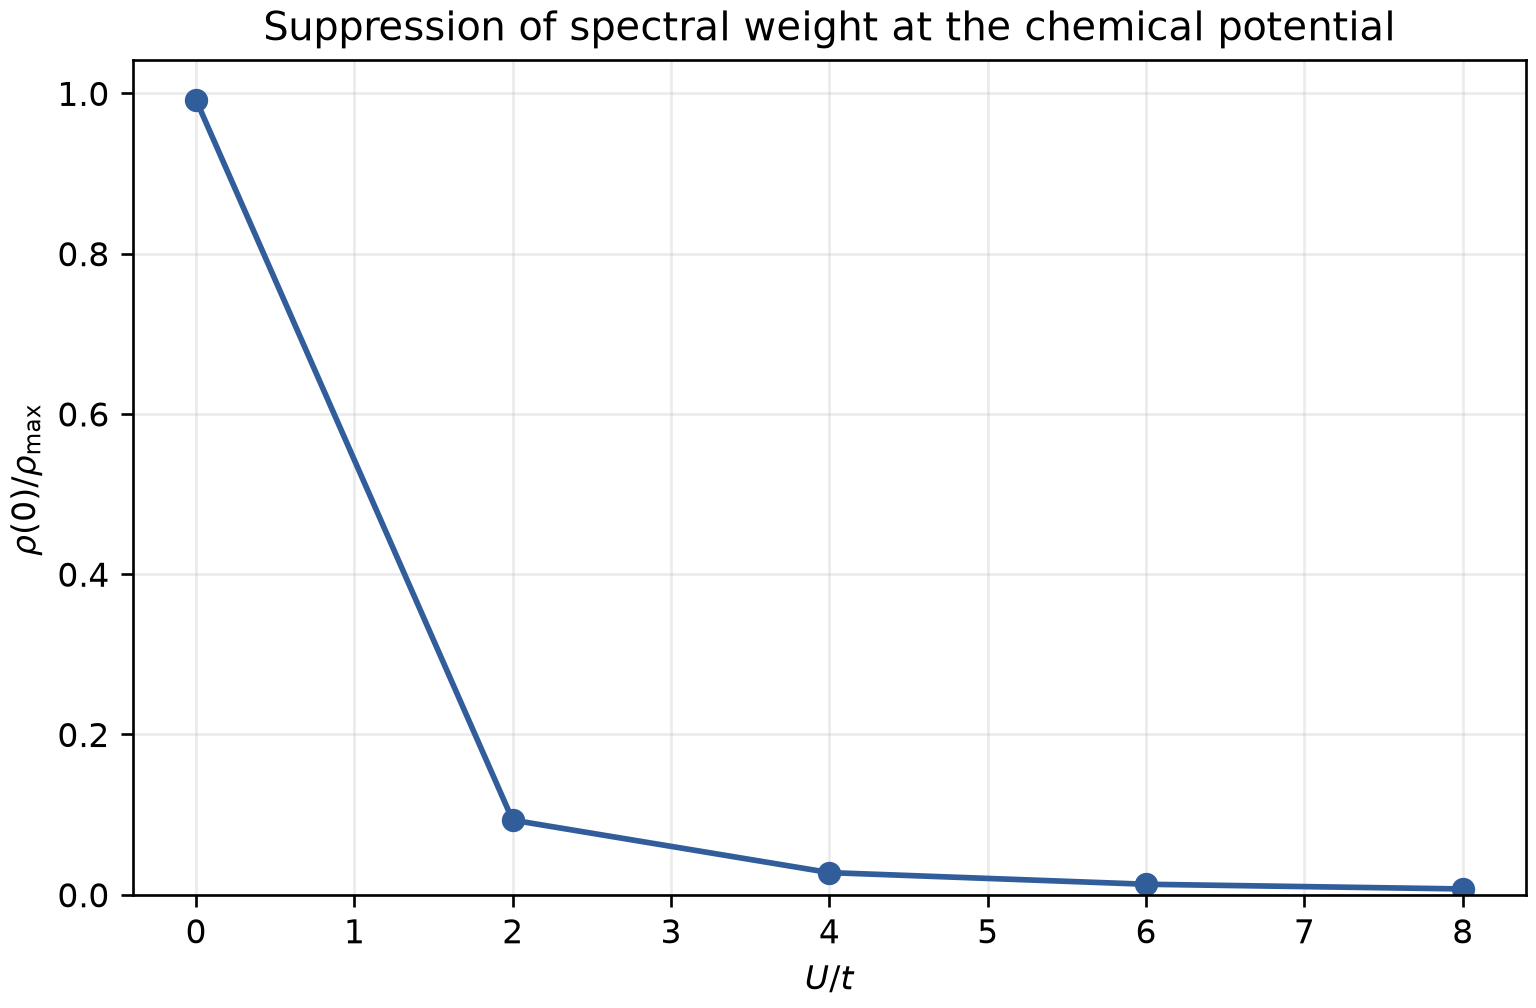
\includegraphics[width=0.82\textwidth]{rho_zero_ratio_vs_U.png}
\caption{$\rho(0)/\rho_{\max}$ 随相互作用强度 $U$ 的变化。}
\end{figure}

\subsection{Krylov 维数收敛}

最低 Ritz 值随 Krylov 维数单调不升。$L=60$ 时能量误差为
$4.832\times10^{-13}$。谱形的 $1.006\times10^{-2}$ 是 $L=60$ 与同一初始
向量产生的 480 步完全再正交参考链之间的相对最大差异，属于保守的自参照
收敛指标，并非相对于精确谱的严格误差。若参考链已进入收敛区，真实谱形误差
应更小。能量只要求逼近一个极端本征值，而谱形需要同时逼近整个能窗内的多个
极点及其权重。

\begin{figure}[H]
\centering
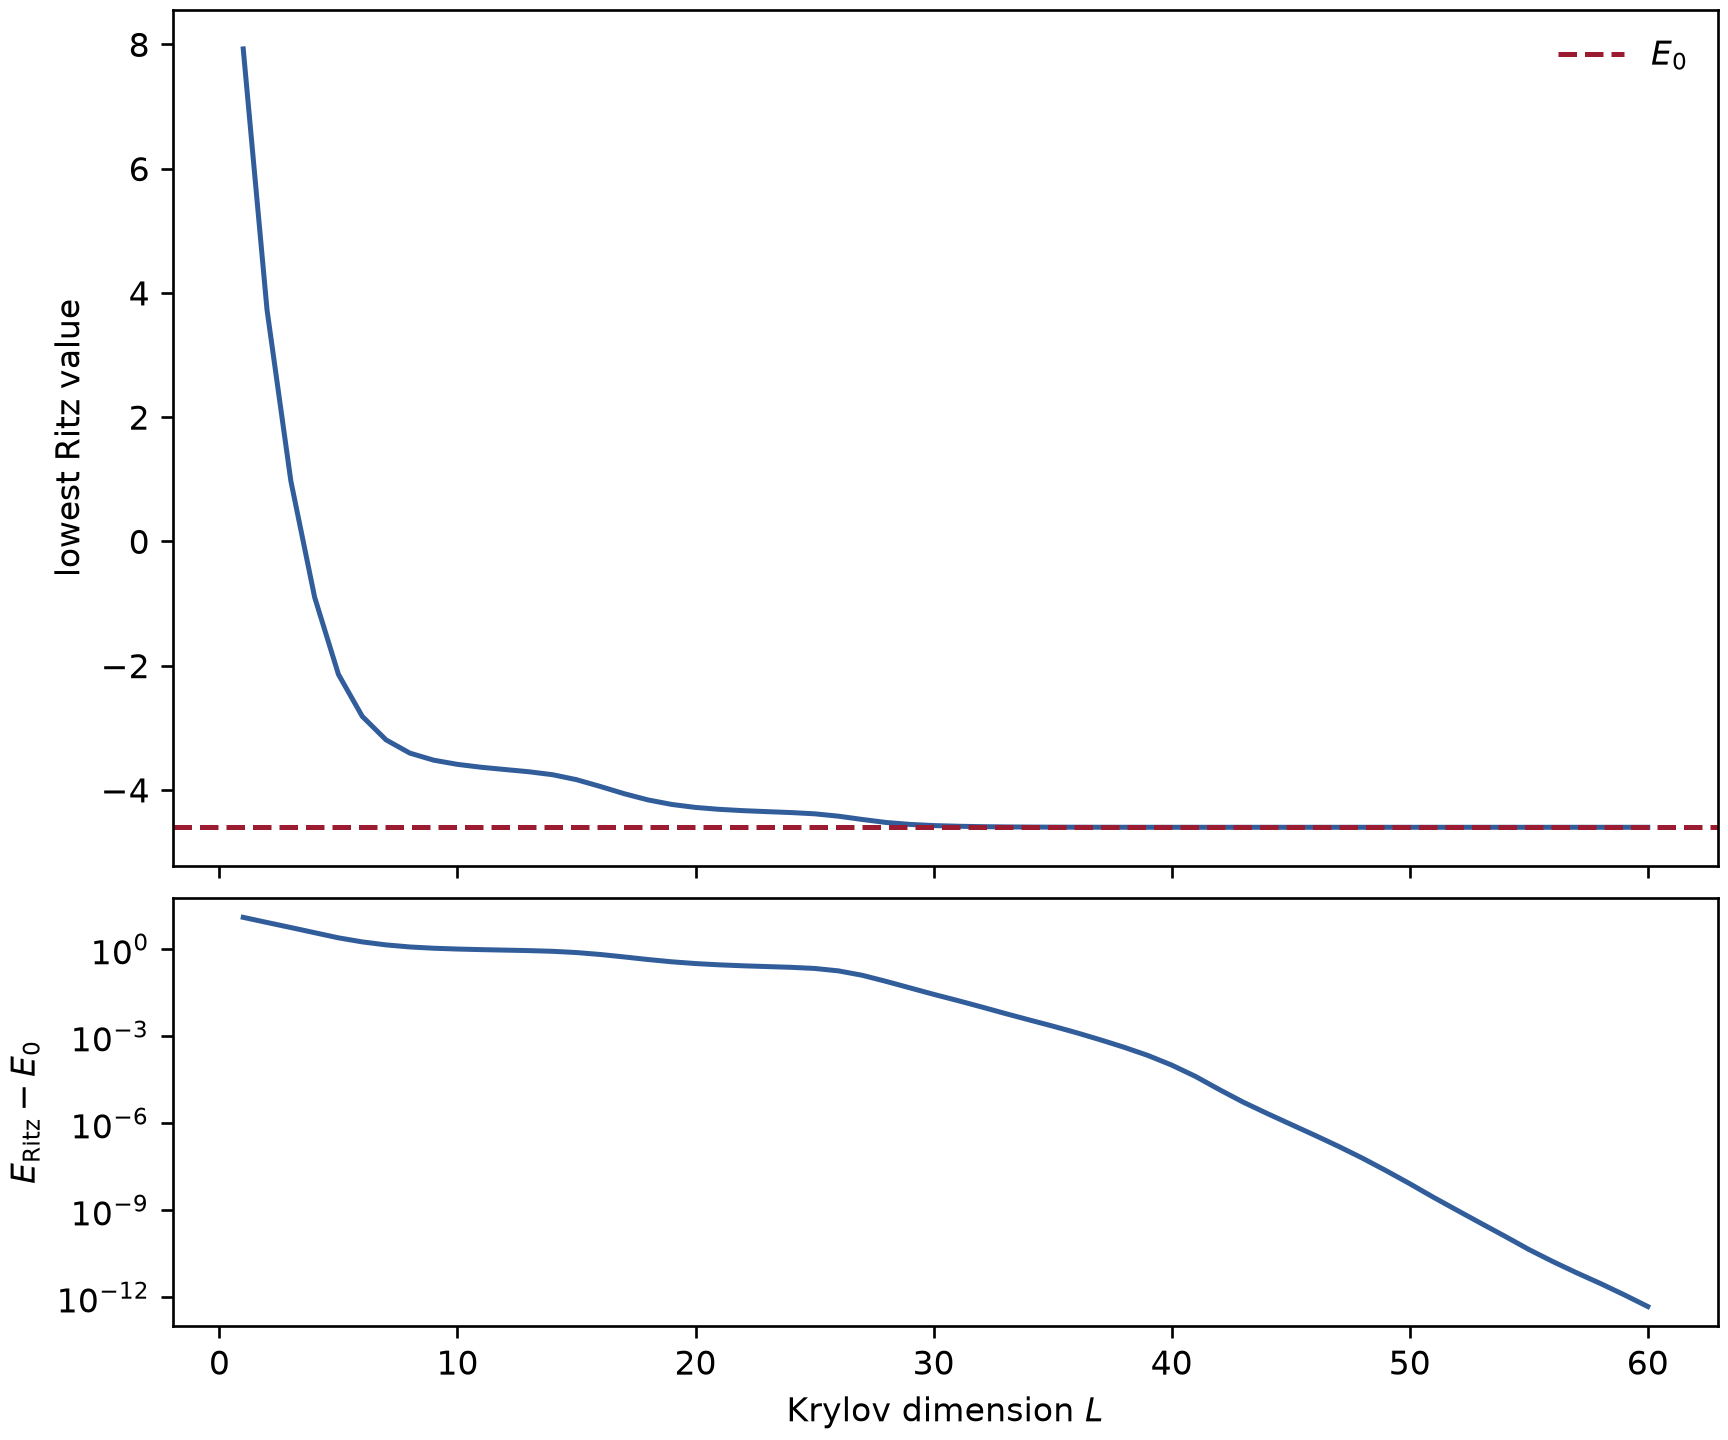
\includegraphics[width=0.92\textwidth]{ritz_convergence.png}
\caption{最低 Ritz 值和能量误差随 Krylov 维数的收敛。}
\end{figure}

\section{校检清单与故障注入}

本次共执行 24 项自动测试和 30 条结果校检，全部通过。主要校检如下：

\begin{longtable}{p{4.2cm}p{4.5cm}p{3.2cm}p{1.6cm}}
\toprule
校检 & 针对错误 & 实测 & 结论 \\
\midrule
\endfirsthead
\toprule
校检 & 针对错误 & 实测 & 结论 \\
\midrule
\endhead
分块维数 & 基底漏项或重复 & 4900 & \good \\
matrix-free / CSR & 跳跃符号、边界、索引、$U$ 项 & $1.249\times10^{-16}$ & \good \\
厄米性 & 反向跳跃缺失或符号不对称 & 0 & \good \\
相互作用 trace & $U$ 项缺失或计数错误 & 39200 & \good \\
基态残差 & 本征求解未收敛 & $1.544\times10^{-14}$ & \good \\
Lanczos 正交性 & 归一化或再正交错误 & $6.850\times10^{-16}$ & \good \\
Lanczos 完整递推 & $a,b$ 下标或末端项错误 & $8.262\times10^{-15}$ & \good \\
连分数 / 直接求解 & 递推方向、最深层或起始向量 & $1.133\times10^{-9}$ & \good \\
加谱权重 & 产生算符、目标块或 $\alpha^2$ & $w_{\rm add}=8$ & \good \\
减谱权重 & 湮灭算符、目标块或 $\alpha^2$ & $w_{\rm rem}=8$ & \good \\
$U=0$ 解析谱 & $t$、边界、$\eta$、归一化与连分数 & $8.667\times10^{-14}$ & \good \\
加减谱逐点镜像 & $\mu$ 或两半谱频率符号 & 最大 $3.382\times10^{-7}$ & \good \\
Ritz 变分单调性 & Krylov 更新或 $T$ 错误 & 违反量 0 & \good \\
\bottomrule
\end{longtable}

故障注入进一步证明校检具有辨别力：翻转跳跃符号使随机向量作用相对差达到
$0.6681$；删除周期边界键产生 $0.1175$ 的相对差；删除 $U$ 项使 trace 偏差
达到 $39200$。完整逐条记录位于
\begin{center}
\path{output/data/validation_checklist.csv}
\end{center}

\section{复现信息与结论}

\begin{table}[H]
\centering
\begin{tabular}{p{5.2cm}p{9cm}}
\toprule
项目 & 值 \\
\midrule
Python & 3.14.7 \\
NumPy / SciPy / Matplotlib & 2.5.3 / 1.18.1 / 3.11.2 \\
随机种子 & 20260928 \\
频率网格 & $[-10,10]$，2001 点 \\
谱 Lanczos 上限 & 240 \\
直接 resolvent 对比上限 & 480 \\
谱形参考链 & 480 步，完全再正交 \\
本征求解 / 简并容差 & $10^{-11}/10^{-8}$ \\
\bottomrule
\end{tabular}
\end{table}

固定粒子数分块把问题压缩到可管理的 4900 维主块；Lanczos 三对角化同时提供
低能 Ritz 值和 Green 函数连分数。$U=0$ 解析基准达到
$8.667\times10^{-14}$ 的峰值归一误差。在 $U=4$ 时基态唯一，$\mu=2$，
加、减谱权重均为 8。随 $U$ 增大，化学势附近谱权重受到显著压制，有限尺寸谱
呈现清楚的上下 Hubbard 带结构。

除题目最低要求外，还完成加减谱逐点粒子-空穴校检、相互作用 trace 组合恒等式、
三种故障注入，以及能量与谱形的 Krylov 收敛对比。完整数值结果集中记录在
\code{output/result.md} 中。

\vspace{1em}
\noindent\colorbox{lightblue}{\parbox{0.94\textwidth}{
\textbf{AI 使用记录说明：}本报告汇总已经测试的物理与数值结果。完整真实对话
记录与修改日志见 \code{AI\_USAGE\_RECORD.md}。}}

\end{document}

